\documentclass[11pt]{article}

\usepackage[margin=1in]{geometry}
\usepackage{amsmath,amssymb}
\usepackage{booktabs,longtable,array}
\usepackage{graphicx}
\usepackage{microtype}
\usepackage{xcolor}
\usepackage{hyperref}
\usepackage{enumitem}

\hypersetup{
  colorlinks=true,
  linkcolor=blue!55!black,
  citecolor=blue!55!black,
  urlcolor=blue!55!black,
  pdftitle={Supplemental Material: From a Free-Boundary MOTS Saddle-Node to a Spacelike Marginal Tube in Dynamical Five-Dimensional Gravity},
  pdfauthor={Ronald Bibb},
  pdfsubject={Validation and reproducibility record for a free-boundary MOTS saddle-node and spacelike marginal tube},
  pdfkeywords={braneworld; marginally outer trapped surface; free boundary; saddle-node bifurcation; dynamical horizon; numerical relativity; supplemental material}
}
\setlist{nosep}
\newcommand{\MOTS}{\mathrm{MOTS}}
\newcommand{\dd}{\mathrm{d}}
\newcommand{\PASS}{\textsc{pass}}
\newcommand{\FAIL}{\textsc{fail}}
\newcommand{\II}{\mathrm{II}}
\newcolumntype{L}[1]{>{\raggedright\arraybackslash}p{#1}}

\title{Supplemental Material for\\
``From a Free-Boundary MOTS Saddle-Node to a Spacelike Marginal Tube\\
in Dynamical Five-Dimensional Gravity''}
\author{Ronald Bibb\\
\small Independent Researcher, Lilburn, Georgia, USA\\
\small Correspondence: \texttt{ronbibb@gmail.com}}
\date{28 August 2026}

\begin{document}
\maketitle

\section{Purpose and evidentiary scope}

This supplement gives the definitions, acceptance criteria, extended
numerical results, negative studies, and reproducibility structure underlying
the article's two linked inferences.  First, an independently constructed
G9/G10/G11 parent sequence evolves from no accepted upper-brane-capped
marginally outer trapped surface (MOTS) to two opposite-stability branches,
and pseudo-arclength continuation resolves their common critical surface.
The principal zero mode, endpoint-eliminated discrete-adjoint coefficients,
and invariant one-half area law establish a finite-resolution free-boundary
MOTS saddle-node in the $SO(3)$-symmetric sector.  An independent G10
half-timestep evolution repeats the complete critical analysis.

Second, the stable outer branch is followed over a fixed post-fold interval.
Its leaves form a future-outward spacelike marginal tube with negative inward
expansion, increasing area, positive principal stability, and orthogonal brane
contact.  The causal character and geometry transfer across G9/G10/G11 and an
independent G10 half-timestep evolution.  A reflected, brane-inclusive
quasi-local charge ledger closes locally and over a finite segment.  This
supports a finite-resolution free-boundary dynamical-horizon-segment
interpretation in the selected symmetry sector and foliation
\cite{AshtekarKrishnan2002,AshtekarKrishnan2003}.

The saddle-node mechanism itself is established theory
\cite{BoothCoxOkpala2026}; it is not claimed as a new mechanism.  The combined
result is numerical and quasi-local.  It is not an event-horizon
reconstruction, a proof excluding every possible initial marginal surface, a
continuum theorem, a nonlinear-stability theorem, or a global mass or
source-ownership ledger.  It also does not determine the nonsymmetric
nonprincipal spectrum.  Those exclusions are part of the result's scope, not
caveats to be silently relaxed.

The validation record is organized by scientific risk.  Each principal test
has four elements: the alternative explanation being tested, a criterion fixed
before interpretation, the measured outcome, and the consequence for the
claim.  Operational details---hashes, complete runner histories, environment
receipts, and restart records---belong to the reproducibility archive rather
than to the scientific argument.

The novelty claim is correspondingly narrow.  Cigar-shaped apparent horizons
in braneworld initial data and dynamically formed brane-intersecting horizons
in RSII precede this work \cite{ShiromizuShibata2000,WangChoptuik2016}, and
MOTS pair creation is already classified as a saddle-node bifurcation
\cite{BoothCoxOkpala2026}.  Free-boundary MOTS stability, rigidity, and
higher-dimensional structure likewise have an established mathematical
literature
\cite{AlaeeLesourdYau2020,Chai2024,Mendes2021,Lee2025,deAlmeidaMendes2026}.
Free-boundary minimal annuli also provide a neighboring static fold and
Jacobi--Robin degeneration result \cite{Pigazzini2026}; that setting does not
evaluate the dynamical MOTS adjoint transversality and quadratic coefficients
tested here.
The unresolved issue addressed here is whether the complete local fold
hypotheses are realized when a physical contact condition enters the MOTS
boundary-value map and the ambient geometry is supplied by a nonlinear
evolution.

The contribution is therefore the closed numerical chain: the physical Robin
domain, branch connection, simple principal zero mode, nonzero
endpoint-eliminated discrete adjoint projections, invariant square-root
separation, three-grid spatial closure, and an independent half-timestep
comparison.  The stabilized compact braneworld supplies the concrete
five-dimensional realization.  One such realization establishes that the
physical boundary does not obstruct the local fold structure in this problem;
it does not establish genericity, a universal theorem, or a new bifurcation
mechanism.

\section{Model, fields, and conventions}

The bulk model is five-dimensional Einstein gravity with
$\Lambda_5=-6/\ell^2$ on the doubled $S^1/\mathbb{Z}_2$ cover.  The numerical
domain is the fundamental compact interval with fixed branes at its endpoints.
The matter sector contains a Goldberger--Wise stabilizer $\Phi$ and an
independent collapse scalar $\chi$
\cite{RandallSundrum1999,GoldbergerWise1999,DeWolfeFreedmanGubserKarch2000,TanahashiTanaka2011}:
\begin{align}
S={}&\frac{1}{2\kappa_5^2}\int\dd^5x\sqrt{-g}\,(R-2\Lambda_5)
-\sum_i\int_{\Sigma_i}\dd^4x\sqrt{-h_i}\,[\lambda_i+U_i(\Phi)]
\nonumber\\
&-\frac12\int\dd^5x\sqrt{-g}\left[(\nabla\Phi)^2+m_\Phi^2\Phi^2
+(\nabla\chi)^2+m_\chi^2\chi^2\right],
\end{align}
with $U_i(\Phi)=\gamma_i(\Phi-v_i)^2/2$.  The induced metric obeys the
oriented Israel conditions, the stabilizer obeys the action-derived scalar
wall condition, and $\chi$ obeys reflecting Neumann data.  The computation
retains the stabilizer response; it does not integrate out the radion.
The displayed action is the doubled-cover thin-shell action.  An equivalent
one-sided interval variational principle includes the appropriate
Gibbons--Hawking--York terms and doubles the one-sided bulk contribution
relative to each brane action
\cite{Israel1966,GibbonsHawking1977,BattyeCarter2001}.  With outward normals it yields
\begin{equation}
K^{(B)}_{\mu\nu}=\frac{\kappa_5^2}{2}
\left(S_{\mu\nu}-\frac13 S h_{\mu\nu}\right),
\qquad n^a_{\rm out}\nabla_a\Phi=-\frac12 U_i'(\Phi),
\end{equation}
which is the sign and factor convention implemented at both interval walls.

We impose $SO(3)$ symmetry in the three noncompact spatial directions while
retaining dependence on areal radius $r$ and compact coordinate $z$.  Initial
data are momentarily time symmetric,
\begin{equation}
K_{ij}=0,\qquad \Pi_\Phi=0,\qquad \Pi_\chi=0,
\end{equation}
and contain a smooth reflection-adjusted scalar pulse localized near the upper
brane.  The primary datum is the family member labelled $A=7.90$.  The label is
a numerical family coordinate, not an invariant critical parameter.

Table~\ref{tab:model-parameters} gives the dimensionless parameters needed to
identify the reported family.  We use $\ell=\kappa_5=1$, so the compact
coordinate spans $z\in[1,e]$.  The load-bearing repaired G9/G10/G11 line uses
$r/\ell\in[0,10]$.  The superseded pre-repair G7/G8 trajectory, retained only
as a historical record below, used $r/\ell\in[0,8]$.
The stabilizer targets are $v_0=\sqrt{0.01}$ and
$v_1=v_0e^{-0.1}$, and $m_\Phi^2=0.1(4.1)=0.41$.  The wall tensions are
retuned consistently with the finite-stiffness background solve rather than
held at their unstabilized values.

\begin{table}[ht]
\centering
\caption{Primary dimensionless model and discretization parameters.}
\label{tab:model-parameters}
\begin{tabular}{@{}ll@{}}
\toprule
Quantity & Value \\
\midrule
$\ell$, $\kappa_5$, compact separation $d/\ell$ & $1$, $1$, $1$ \\
$\epsilon$, Goldberger--Wise backreaction, $m_\Phi^2$ & $0.1$, $0.01$, $0.41$ \\
wall stiffness $\gamma\ell$ & $20$ \\
wall targets $v_0,v_1$ & $0.1$, $0.0904837418036$ \\
retuned bare tensions $\lambda_0,\lambda_1$ & $5.9999903768$, $-6.0528442777$ \\
background warp slopes $\beta_0,\beta_1$ & $1$, $1.00880714399$ \\
background proper separation$/\ell$ & $0.9996389584$ \\
collapse-scalar mass $m_\chi^2$ & $0$ \\
pulse amplitude $A$, radial width $\sigma_r$ & $7.90$, $1$ \\
compact-log width $\sigma_y$, center $y_c/d$, images & $0.2$, $0.9$, $5$ \\
historical pre-repair domain and grids & $R_{\max}/\ell=8$; G7 $81\times121$, G8 $97\times145$ \\
repaired critical-sequence domain & $R_{\max}/\ell=10$ \\
repaired critical grids & G9 $113\times211$, G10 $129\times241$, G11 $145\times271$ \\
critical and half-step $\Delta t/\ell$ & $3.125\times10^{-5}$, $1.5625\times10^{-5}$ \\
background solve tolerance & $10^{-10}$ \\
\bottomrule
\end{tabular}
\end{table}

The background values in Table~\ref{tab:model-parameters} are the sealed
binary64 parent values; the last quoted digits of $\beta_1$, the upper-wall
tension, and the proper separation vary below $7\times10^{-13}$,
$5\times10^{-13}$, and $3\times10^{-10}$, respectively, between the two
archived parent resolutions.  These numerical values, rather than only their
analytic target formulas, are included in the replay package.

For a spatial-slice unit normal $u^a$ and outward surface normal $s^a$, the
outgoing null normal is $\ell_+^a=u^a+s^a$ and
\begin{equation}
\theta_+=D_i s^i+K_{ij}s^is^j-K.
\end{equation}
A MOTS satisfies $\theta_+=0$.  An upper-brane-capped surface closes regularly on the
axis and meets the upper brane orthogonally.  Orthogonal contact with the
support hypersurface is the free-boundary condition used in the cited
literature, and it is precisely the brane endpoint condition imposed here.
The cap is therefore a brane-terminating free-boundary surface; free-boundary and
capillary MOTS stability have an independent mathematical literature
\cite{AlaeeLesourdYau2020,Chai2024,Mendes2021,Lee2025,deAlmeidaMendes2026}, while higher-dimensional MOTSs
have also been treated directly \cite{PaetzSimon2013}.  Linear stability is defined by
\begin{equation}
L f=\delta_{f s}\theta_+.
\end{equation}
In the convention used here, a nonnegative principal eigenvalue is
outward-stable.  The evolved-slice operator is treated as non-self-adjoint.
The interpretation follows the local MOTS-stability framework of
Refs.~\cite{AnderssonMarsSimon2005,AnderssonMarsSimon2008,AnderssonMarsMetzgerSimon2009,PookKolbEtAl2019}.
For the connected cap, the scalar stability operator is strongly elliptic,
and its Robin domain commutes with $SO(3)$.  Free-boundary
principal-eigenvalue theory supplies a positive eigenfunction that is unique
up to scale \cite{AlaeeLesourdYau2020,deAlmeidaMendes2026}.  A group transform
is therefore the same normalized principal eigenfunction.  The symmetric
computation captures the full principal eigenvalue and its simple kernel,
although it does not determine the nonsymmetric nonprincipal spectrum.

The perturbation class is not left implicit.  Writing a nearby cap as
$\rho(\vartheta)+\delta\rho(\vartheta)$, smooth-axis closure and preservation
of orthogonal wall contact impose
\begin{equation}
\partial_\vartheta\delta\rho=0
\quad\hbox{at}\quad \vartheta=0,\pi/2.
\end{equation}
The operator acts on physical normal displacement
$f=w\delta\rho$, where $w=s_Ae_\rho^A>0$.  Hence the implemented condition is
$\partial_\vartheta(f/w)=0$, a homogeneous Robin condition for $f$ when $w$
is nonconstant.  The endpoints are eliminated with seven-point local finite
differences before the unsymmetrized right-eigenvalue problem is solved.  This
boundary treatment is checked by the manufactured Robin spectrum, endpoint
defects below $10^{-10}$, and the 49/65/81-node sequences.  No alternative
stencil-width study is claimed.

\section{Initial-data and search protocol}

\subsection{Bounded initial search}

The load-bearing absence datum is the repaired G9/G10/G11 search at
$t/\ell=0.001$ described in Sec.~\ref{sec:repaired-preformation}; it is followed
by exactly two admitted surfaces at $t/\ell=0.0015$ on those same parent lines.
The earlier searches summarized in this subsection were performed during the
superseded pre-repair study and are preserved only to document how the repaired
calculation was motivated.  They are not independent confirmation of the
repaired result.  Within that historical record, ``no initial MOTS'' means
``no accepted surface in the prespecified bounded search,'' not an analytic
nonexistence theorem.
The principal initial class consists of $C^2$, axisymmetric, star-shaped
upper-brane-capped polar graphs
\begin{equation}
z=z_B-\rho(\vartheta)\cos\vartheta,\qquad
r=\rho(\vartheta)\sin\vartheta,
\end{equation}
with $0\leq\vartheta\leq\pi/2$,
$\rho'(0)=\rho'(\pi/2)=0$, and
$0.10\leq\rho(\vartheta)\leq1.67$.  Separate bounded searches cover
opposite-side capped, closed-star-shaped, and interval-spanning candidates.
Acceptance requires finite geometry, admissible domain and endpoint behavior,
a residual below the fixed tolerance, and repeated recovery under the
specified seed families.

For the historical $A=7.90$ datum, the initial upper-brane-capped searches
return no accepted surface.  The same is true for the five-point R8 sample
$A=7.84,7.86,7.88,7.90,7.92$.  An adverse $A=7.94$ control recovers its known
initial pair.  On each separately constraint-solved G9 and G10 initial slice,
a regular-axis shooting audit samples 2,049 uniformly spaced axis radii across
$[0.10,1.67]$.  The independently minimized brane residual stays positive,
$0.0280624085$ on G9 and $0.0282193410$ on G10, under twelve cutoff,
tolerance, and step variations.  The same implementation resolves both nearby
$A=7.94$ control roots to residuals of order $10^{-13}$.  The grade remains a
strong floating-point no-root result rather than an interval or degree proof:
an arbitrarily narrow unsampled root island is not mathematically excluded.

\subsection{Surface representations}

On the historical pre-repair trajectory, the primary evolved-surface
representation uses the fixed twelve-seed bank
$1.15,1.20,\ldots,1.70$.  Every seed is solved at 40 and 48 cosine modes on
257 collocation points, with expansion target $5\times10^{-4}$.  A candidate
requires two-mode convergence in-domain below condition number $10^5$, full
profile and endpoint agreement within $0.2\%$, and an independent 513-point
expansion below $0.002$; signatures within $0.005$ are deduplicated.  The
confirmation representation is an independently
parameterized local boundary-value problem.  Acceptance requires agreement in
branch count, endpoint geometry, and proper cap area.  Both representations
operate on the same evolved spacetime, so their agreement constrains detector
and parameterization error but is not an independent evolution.

The $10^5$ condition-number ceiling belongs only to that historical spectral
detector.  The load-bearing repaired search and critical continuation below
use the distinct local second-order BVP and
does not call or inherit that ceiling; its admission uses the local residual,
endpoint slope, physical domain, and independent expansion cross-check.
Accordingly, proximity to the principal zero cannot remove a continuation
point through the spectral-detector condition gate.  No critical
condition-number trace was archived, and none is used as evidence for the
saddle-node classification.

The BVP detector solves the local second-order cap equation with
$\rho'(0)=\rho'(\pi/2)=0$ from the same twelve scalar seeds.  Admission
requires local interior expansion below $2\times10^{-4}$, endpoint-slope error
below $2\times10^{-4}$, and a cross-check by the primary expansion evaluator
below $0.002$.  Its flat-slice control reproduces the analytic marginal
half-sphere radius $1.25$ to $3.91\times10^{-11}$ relatively and gives an
independent expansion maximum $3.66\times10^{-6}$.

In the historical pre-repair record, at $t=0.000625$, $0.001$, and $0.004$,
each G7/G8 grid yields exactly two accepted branches, with six seed recoveries
per branch.  The largest
shooting/BVP endpoint mismatch is $0.04764\%$ and the largest cross-grid BVP
endpoint transfer is $0.23205\%$.

\section{Evolution and ordered acceptance gates}

The Einstein--scalar system is evolved in a regular $SO(3)$-reduced
generalized-harmonic formulation \cite{Pretorius2005}.  Compact-wall rows own the wall conditions;
axis regularity owns interior-axis rows; wall--axis and wall--outer corners use
an explicitly staged ownership policy.  The canonical policy is the scientific
path, while an independent wall-owner policy is retained as a control.

The ordered gate structure prevents a later geometric observation from
overriding an earlier invalid computation:
\begin{enumerate}
\item runtime, source, and input identity;
\item finite values, signature, and physical admissibility;
\item compact-wall, axis, corner, and ownership identities;
\item repeated deterministic replay;
\item temporal refinement and endpoint consistency;
\item spatial field and physical-tensor closure;
\item horizon count, geometry, and stability interpretation.
\end{enumerate}
An audit or determinism failure is not relabelled as a scientific negative
result.  A resource stop carries no scientific inference.

\section{Formation, geometry, and stability}

\subsection{Free-boundary stability condition}

Let $\varrho$ be the outward unit normal to the brane within the spatial
slice, $N$ the unit normal to the MOTS, and $\nu$ the outward conormal to its
boundary.  Orthogonal contact gives $\nu=\varrho$ and
$g(N,\varrho)=0$.  For a physical normal variation $fN$, varying this
orthogonality relation gives the free-boundary operator
\begin{equation}
Bf=\nabla_\nu f-\II^{\partial M}(N,N)f=0.
\end{equation}
Thus the brane-extrinsic-curvature term is part of the physical problem.

For the implemented upper-brane cap, the compact endpoint lies on the upper wall
$z=e$.  The retained interval lies toward decreasing $z$, so its outward wall
normal is $\varrho=h_{zz}^{-1/2}\partial_z$.  We choose the outward cap
conormal $\nu=\varrho$, the MOTS normal toward increasing areal radius,
$N=h_{rr}^{-1/2}\partial_r$, and
$\II^{\partial M}(X,Y)=g(\nabla_X\varrho,Y)$.  Wall parity gives
$h_{zr}=0$.  With these fixed orientations, the physical
normal amplitude associated with a coordinate graph displacement
$\delta\rho$ is $f=w\delta\rho$ with $w=\sqrt{h_{rr}}$.  The same geometry
gives
\begin{equation}
\II^{\partial M}(N,N)=\frac12\nu(\log h_{rr})=\nu(\log w),
\qquad Bf=w\nu(\delta\rho).
\end{equation}
Consequently the implemented endpoint condition
$\partial_\vartheta\delta\rho=0$, equivalently
$\partial_\vartheta(f/w)=0$, is the coordinate reduction of the physical
Robin condition; it does not omit the brane-curvature contribution.  The
zero derivative at the axis is separately the smooth-axis regularity
condition.

\subsection{Three-grid formation comparison}

The primary repaired critical line is independently constructed on G9
$113\times211$, G10 $129\times241$, and G11 $145\times271$.  The prescribed
surface search accepts no branch at $t/\ell=0.001$ and exactly two at
$t/\ell=0.0015$ on every grid.  All endpoint, proper-geometry, principal-sign,
operator-resolution, and Robin-boundary gates pass.  The direct observables
are listed in Table~\ref{tab:supp-three-grid}.

\begin{table}[ht]
\centering
\caption{Three-grid repaired-parent surface observables at $t/\ell=0.0015$.}
\label{tab:supp-three-grid}
\begin{tabular}{@{}lrrrr@{}}
\toprule
grid & $\mathcal A_{\rm in}$ & $\lambda_{\rm in}$ & $\mathcal A_{\rm out}$ & $\lambda_{\rm out}$ \\
\midrule
G9  & $40.67520320$ & $-0.25894888$ & $40.72845794$ & $+0.29347891$ \\
G10 & $40.67520099$ & $-0.25895908$ & $40.72845823$ & $+0.29348687$ \\
G11 & $40.67519977$ & $-0.25896247$ & $40.72845818$ & $+0.29348984$ \\
\bottomrule
\end{tabular}
\end{table}

For G9--G10, the maximum endpoint, geometry, and relative-eigenvalue
differences are $1.022\times10^{-6}$, $1.764\times10^{-7}$, and
$3.938\times10^{-5}$, respectively.  For G10--G11 they are
$6.529\times10^{-7}$, $1.177\times10^{-7}$, and
$1.311\times10^{-5}$.  Thus the repaired line's earlier absence at
$t/\ell=0.001$ is a pre-formation datum, not a permanent failure to form the
pair.

\subsection{Pseudo-arclength continuation and zero bracket}

Starting from the outer branch at $t/\ell=0.0015$, time is promoted to an
unknown of the local cap BVP and an integral pseudo-arclength condition is
added \cite{Keller1977}.  The spacetime state between exact RK2 endpoints uses the fixed dense
extension
\begin{equation}
y(\theta)=y_n+\Delta t[(\theta-\theta^2)k_1+\theta^2k_2],
\qquad \theta=(t-t_n)/\Delta t .
\end{equation}
Every replayed endpoint is bitwise identical to the stored evolution.  Each
accepted continuation point starts from arclength step $1/64$ and permits only
the prespecified dyadic backoff through $1/4096$; zero-bracket refinement has
the technical floor $1/65536$.  The augmented BVP uses 121 initial angular
nodes, relative tolerance $2\times10^{-6}$, at most 6,000 adaptive nodes, and
a 501-node dense output.  An accepted corrector must also have absolute
arclength residual at most $2\times10^{-5}$ before the fixed-time surface is
re-solved and passed through the inherited local and cross-evaluator gates.

The principal eigenvalue first changes sign and remains resolved under
bracket refinement.  Table~\ref{tab:supp-critical} reports the final bracket
and near-critical discrete data.  The displayed $\lambda_*$ and coefficients
are evaluated at the smaller-magnitude endpoint of the final bracket rather
than at an exact floating-point kernel.

\begin{table}[ht]
\centering
\caption{Three-grid critical-time estimate and near-critical discrete operator
and normal-form data.  $\mathcal A_{\rm nc}$ is evaluated at the selected
bracket endpoint rather than an exact critical surface.}
\label{tab:supp-critical}
\begin{tabular}{@{}lrrr@{}}
\toprule
quantity & G9 & G10 & G11 \\
\midrule
$t_*/\ell$ & $0.0011725421$ & $0.0011725452$ & $0.0011725359$ \\
time-bracket width & $1.8426\times10^{-7}$ & $1.7177\times10^{-7}$ & $1.8667\times10^{-7}$ \\
$\mathcal A_{\rm nc}$, one-sided & $40.70345140$ & $40.70336590$ & $40.70344580$ \\
$\lambda_*$ & $-7.3854\times10^{-4}$ & $-1.6944\times10^{-3}$ & $-7.8666\times10^{-4}$ \\
next reduced-sector eigenvalue & $5.56598$ & $5.56531$ & $5.56595$ \\
imposed $f_L^*f_R$ & $1.0000000$ & $1.0000000$ & $1.0000000$ \\
near-critical $a=\langle f_L,\partial_t\theta_+\rangle$ & $-20.76513$ & $-20.76565$ & $-20.76493$ \\
near-critical $b=\tfrac12\langle f_L,\partial_{f_R}^2\theta_+\rangle$ & $2.80717$ & $2.80410$ & $2.81060$ \\
\bottomrule
\end{tabular}
\end{table}

The mode convention is exact.  The Robin endpoint rows are first eliminated,
so the stability matrix acts on physical normal displacement $f$ at the
interior uniform $\vartheta$ nodes.  Its right eigenvector is phased so that
the component of largest modulus is positive real and then scaled to
$\|f_R\|_\infty=1$.  The left vector is the Euclidean
conjugate-transpose eigenvector of that reduced matrix, not a mass-matrix
adjoint or a separately discretized formal continuum adjoint.  It is scaled
afterward to $f_L^*f_R=1$.  Thus the reported unit overlap is a construction
identity, not an additional nondegeneracy observation.  Before rescaling, the
code requires only that the overlap magnitude exceed $10^{-14}$; that value
was not archived.  The endpoint behavior of $f_R$ is restored through the
same Neumann extension that implements the Robin graph condition.  The
near-critical coefficient magnitudes and individual signs are reproducible
under this discrete orientation convention, while their nonvanishing is the
normal-form conclusion.
An admissible change of eigenvector normalization rescales $a$ and $b$ by
finite nonzero factors; it changes their numerical magnitudes but cannot
change whether either coefficient vanishes.

The near-critical principal mode is real and sign-definite on each grid.  The 65--81-node
principal differences lie between $3.59\times10^{-5}$ and
$3.78\times10^{-5}$; the doubled-step differences are approximately
$4.78\times10^{-4}$.  The next mode is more than five units away.  Centered
step halving changes $a$ by at most $1.56\times10^{-9}$ and $b$ by at most
$2.67\times10^{-3}$ without changing either sign.  Relative adjacent-grid
transfers are at most $3.46\times10^{-5}$ for $a$ and
$2.32\times10^{-3}$ for $b$, far below the prospective $0.20$ ceilings.
The G9/G10/G11 sequences for $t_*$, $\mathcal A_{\rm nc}$, $a$, and $b$ are all
nonmonotone.  Their full relative spreads are, respectively,
$7.87\times10^{-6}$, $2.10\times10^{-6}$,
$3.46\times10^{-5}$, and $2.31\times10^{-3}$.  Consequently no real
three-level Richardson order is defined and no continuum-extrapolated value
or uncertainty is inferred.  The evidence is small finite-resolution scatter
plus the independent temporal comparison below.  The isolated near-critical
principal mode and bracketed zero crossing are consistent with a simple
principal critical kernel.  The roles of that kernel, the transversality
coefficient, and the nonzero quadratic term are those of the standard fold
normal form \cite{Kuznetsov2004}.

\subsection{Invariant square-root test}

Both branches are solved at the five prespecified offsets
$t=t_*+(1,2,4,8,16)\Delta t/16$.  A linear fit of
$(\mathcal A_{\rm out}-\mathcal A_{\rm in})^2$ against time gives the results in
Table~\ref{tab:supp-scaling}.  The fitted critical times agree with the
continuation estimates within the frozen temporal criterion.

\begin{table}[ht]
\centering
\caption{Invariant proper-area scaling fits.  The displayed $R^2$ is for the
linear fit of $(\Delta\mathcal A)^2$ against time; the exponent comes from a
separate log--log fit using the critical time inferred by that linear fit.}
\label{tab:supp-scaling}
\begin{tabular}{@{}lrrr@{}}
\toprule
grid & $t_{*,\rm fit}/\ell$ & free exponent $p$ & squared-fit $R^2$ \\
\midrule
G9  & $0.0011725485$ & $0.4959125$ & $0.9999801$ \\
G10 & $0.0011725343$ & $0.4959672$ & $0.9999804$ \\
G11 & $0.0011725265$ & $0.4959590$ & $0.9999803$ \\
\bottomrule
\end{tabular}
\end{table}

All nine per-grid critical gates and both adjacent-grid aggregate gates pass.

The fit-sensitivity audit separates the two fits rather than treating their
statistics as interchangeable.  Holding $t_*$ at the independently obtained
continuation midpoint gives free exponents $0.49644$, $0.49507$, and
$0.49518$ on G9, G10, and G11.  Omitting one offset at a time gives the ranges
$0.49361$--$0.49956$, $0.49187$--$0.49865$, and
$0.49201$--$0.49872$.  Fixing $p=1/2$ and optimizing only the amplitude gives
maximum relative residuals $0.00920$, $0.01173$, and $0.01153$.  These tests
support the half-power classification while showing that the seventh decimal
place of the original free exponent is not an uncertainty estimate.

\subsection{Independent G10 half-timestep comparison}

The three spatial grids use the same RK2 step and dense extension.  A
prospectively frozen G10 calculation therefore halved the step from
$3.125\times10^{-5}$ to $1.5625\times10^{-5}$, reconstructed the parent from
$t/\ell=0.001$ to $0.0015$ in 32 steps, solved both endpoint anchors anew,
replayed the complete half-step trajectory, and repeated every load-bearing
continuation and critical calculation.  Table~\ref{tab:supp-temporal} gives
the result.

\begin{table}[ht]
\centering
\caption{G10 half-timestep comparison.  The $t_*$ entries are zero-bracket
midpoints; their difference is not an uncertainty estimate.  The
$\mathcal A_{\rm nc}$, $a$, and $b$ differences are relative, with
$\mathcal A_{\rm nc}$ evaluated at the selected near-critical endpoint.}
\label{tab:supp-temporal}
\begin{tabular}{@{}lrrr@{}}
\toprule
quantity & full step & half step & difference \\
\midrule
$t_*/\ell$ & $0.001172545169$ & $0.001172544252$ & $9.1732\times10^{-10}$ \\
$\mathcal A_{\rm nc}$ & $40.70336590$ & $40.70340030$ & $8.4495\times10^{-7}$ \\
$a$ & $-20.76564697$ & $-20.76535233$ & $1.4189\times10^{-5}$ \\
$b$ & $2.80409588$ & $2.80435486$ & $9.2348\times10^{-5}$ \\
free exponent $p$ & $0.495967$ & $0.498057$ & --- \\
squared-fit $R^2$ & $0.9999804$ & $0.9999951$ & --- \\
zero-bracket width & $1.7177\times10^{-7}$ & $1.7918\times10^{-7}$ & --- \\
\bottomrule
\end{tabular}
\end{table}

The full- and half-step zero brackets overlap.  Their midpoint shift is
$9.1732\times10^{-10}$, whereas their widths are $1.7177\times10^{-7}$ and
$1.7918\times10^{-7}$; the shift is not an uncertainty estimate for $t_*$.  The
half-step result retains the real sign-definite near-critical principal mode,
reduced-sector spectral gap, nonzero coefficient signs, and area-scaling gate.
Both independently evolved parents also pass the same finite-value, signature,
constraint, wall, axis, and endpoint gates.  This repeat is an indirect check
against a systematic temporal-evolution error; it is not a standalone
constraint-convergence study.  The free exponent moves from $0.495967$ to
$0.498057$, toward the expected one-half value.  Together with the fit-sensitivity
ranges above, that movement is consistent with the residual exponent offset
being dominated by temporal-discretization bias rather than a fitting artifact,
but two time steps do not define a temporal convergence order.
The prospective limits were $\Delta t/64$ for the bracket-midpoint shift,
$1\%$ for the area, $20\%$ for each coefficient, and $0.4\leq p\leq0.6$ in both
runs.  Every comparison passes, so the prescribed decision sequence does not
call for a quarter-step run.

\subsection{Historical pre-repair formation record}

The following G7/G8 trajectory predates the canonical parity repair and is
retained for provenance rather than counted as independent evidence for the
repaired saddle-node.  Both historical grids are empty in the bounded initial upper-brane-capped search and
then contain two accepted branches in the common bracket
\begin{equation}
0.000500<t_{\rm form}\leq0.000625.
\end{equation}
The pair remains accepted at $t=0.001$ and $t=0.004$.  The independent BVP
representation reproduces the zero-to-two transition.  Figure~\ref{fig:supp-formation}
shows the shared formation bracket and the subsequent growth of the proper-area
separation.

\begin{figure}[ht]
\centering
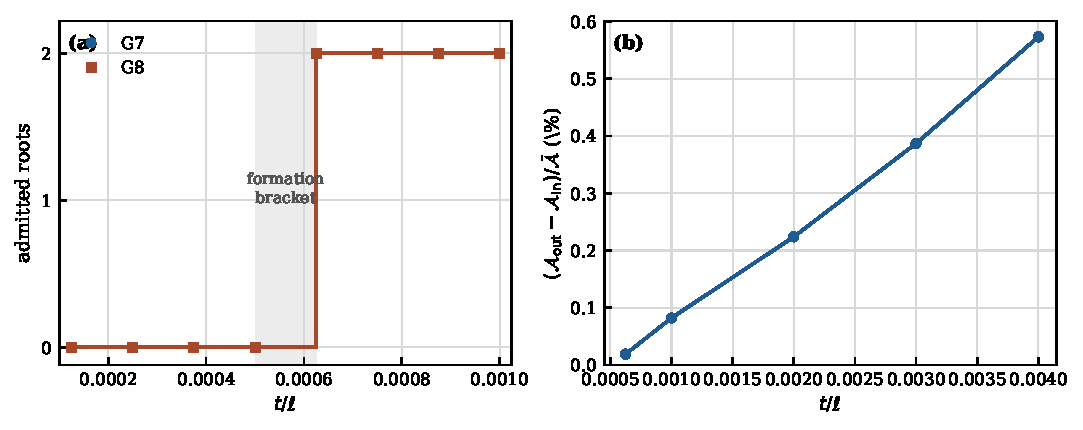
\includegraphics[width=\linewidth]{figures/formation-and-separation.pdf}
\caption{Historical pre-repair realization, retained for provenance and not
used as independent support for the repaired result.  \textbf{Left:} admitted
upper-brane-capped root count on the two G7/G8 grids.  Both histories
change from zero to two in the common formation bracket.  \textbf{Right:}
one-sided proper cap-area separation on G8, shown relative to the mean area at
each sampled time.  The earliest positive gap is not claimed as quantitatively
resolved; the growing separation on later slices is.}
\label{fig:supp-formation}
\end{figure}

\subsection{Historical proper-area separation}

Selected and confirmation proper cap areas agree within $0.0000881\%$; the
individual G7/G8 proper areas agree within $0.0293\%$.  At first detection the
outer-minus-inner gap is $0.02232\%$ on G7 and $0.01908\%$ on G8.  Thus both
grids reproduce the ordering, while the small gap itself differs by about
$16\%$ and is not treated as a precise near-creation observable.  Thereafter
the inner area decreases and the outer area increases.  On G8 the gap grows to
$0.5712\%$ at $t=0.004$, giving a progressively clearer proper-geometric
separation.

\subsection{Historical principal stability spectrum}

The superseded G7/G8 realization also assigned negative principal eigenvalues
to the inner branch and positive values to the outer branch at every sampled
time.  Its full 33/49/65/81-node spectra, Fr\'echet-step comparison,
manufactured control, and numerical values remain in the archive for
provenance but are not used to close the repaired result.  The load-bearing
stability evidence is the direct G9/G10/G11 result and half-timestep
comparison reported above.  Neither realization implies nonlinear basin
stability.

\section{Post-fold marginal-tube construction and controls}

\subsection{Generator, causal character, and area transport}

Let $u^a$ be the future unit normal to a slice and $s^a$ the outward unit
normal to a marginal leaf.  With
\begin{equation}
\ell^a=\frac{u^a+s^a}{\sqrt2},\qquad
n^a=\frac{u^a-s^a}{\sqrt2},\qquad \ell\mathbin\cdot n=-1,
\end{equation}
the normal projection of the positive-time tube generator is
\begin{equation}
X^a=\alpha u^a+v_n s^a=A\ell^a-Bn^a,
\qquad
A=\frac{\alpha+v_n}{\sqrt2},\quad
B=\frac{v_n-\alpha}{\sqrt2},
\label{eq:supp-tube-generator}
\end{equation}
so that $X^2=2AB=v_n^2-\alpha^2$.  A future-outward spacelike tube requires
$A>0$ and $B>0$; a positive norm alone would also admit the opposite
orientation.  The reconstruction therefore retains the signs of $A$, $B$,
and $v_n$ as well as the norm.  Backward, centered, and forward velocity paths
measure the one-sided temporal spread against which the centered norm is
resolved.  Equation~\eqref{eq:supp-tube-generator} fixes the normalization and
orientation used in every causal-signature comparison below.

The numerical reconstruction starts from the meridional embedding
\begin{equation}
x^A_i(\vartheta)=
\left(-\rho_i\cos\vartheta,\rho_i\sin\vartheta\right),
\qquad
S^A_i=\partial_\vartheta x^A_i,
\label{eq:supp-embedding}
\end{equation}
on leaf $i$.  For physical spacing $\Delta\tau$, the three retained coordinate
velocities are
\begin{align}
\dot x^A_{\rm b}&=\frac{x^A_i-x^A_{i-1}}{\Delta\tau},&
\dot x^A_{\rm c}&=\frac{x^A_{i+1}-x^A_{i-1}}{2\Delta\tau},&
\dot x^A_{\rm f}&=\frac{x^A_{i+1}-x^A_i}{\Delta\tau}.
\label{eq:supp-velocity-paths}
\end{align}
The corresponding spacetime vectors are
$V_p^\mu=(1,\dot x^A_p,0,0)$, $p\in\{{\rm b,c,f}\}$.  Removing the component
tangent to the leaf gives the invariant normal-plane signature
\begin{equation}
\Xi_p=g(V_p,V_p)-\frac{g(V_p,S)^2}{g(S,S)}.
\label{eq:supp-causal-signature}
\end{equation}
With signature $(-,+,+,+,+)$, $\Xi_p>0$ is spacelike.  The centered normal
speed in Eq.~\eqref{eq:supp-tube-generator} is reconstructed independently as
$v_n=s_A(\beta^A+\dot x^A_{\rm c})$, where $s_A$ is the unit leaf conormal and
$\beta^A$ the ADM shift.

At each surface node define
\begin{equation}
\delta\Xi=\max\left(
|\Xi_{\rm b}-\Xi_{\rm c}|,
|\Xi_{\rm f}-\Xi_{\rm c}|
\right),
\qquad
m_\Xi=\min_\vartheta\left(|\Xi_{\rm c}|-\delta\Xi\right).
\label{eq:supp-causal-margin}
\end{equation}
A node is resolved only if the three signs agree and
$|\Xi_{\rm c}|>\delta\Xi$.  The full/half comparison uses the pointwise
normalization
\begin{equation}
\epsilon_{\Xi,p}=
\frac{|\Xi^{\Delta t}_p-\Xi^{\Delta t/2}_p|}
{\max(|\Xi^{\Delta t}_p|,|\Xi^{\Delta t/2}_p|,10^{-12})},
\label{eq:supp-causal-temporal-error}
\end{equation}
and takes its maximum over all paths, nodes, and matched leaves.
Equations~\eqref{eq:supp-embedding}, \eqref{eq:supp-velocity-paths},
\eqref{eq:supp-causal-signature}, \eqref{eq:supp-causal-margin}, and
\eqref{eq:supp-causal-temporal-error} therefore define the complete
surface-velocity reconstruction and the two normalizations used for the
causal classification.

Write the full deformation as $\mathcal X^a=X^a+V^a$, with $V^a$ tangent to
the leaf.  The first variation of the one-sided area is
\begin{equation}
\frac{\dd\mathcal A}{\dd\lambda}
=\int_{\mathcal S}
\left(A\theta_{(\ell)}-B\theta_{(n)}\right)\dd A
+\int_{\partial\mathcal S}V\mathbin\cdot\nu\,\dd A_2.
\label{eq:supp-area-transport}
\end{equation}
At orthogonal contact, the leaf conormal $\nu$ is the spatial brane normal.
Because the endpoint moves within the brane,
$\mathcal X\mathbin\cdot\nu=0$, while
$X\mathbin\cdot\nu=0$ by normality to the leaf.  Hence
$V\mathbin\cdot\nu=0$.  On an exact marginal tube,
\begin{equation}
\frac{\dd\mathcal A}{\dd\lambda}
=-\int_{\mathcal S}B\theta_{(n)}\,\dd A,
\label{eq:supp-area-law}
\end{equation}
so $B>0$ and $\theta_{(n)}<0$ imply strict area increase.  This is the
free-boundary version of the local dynamical-horizon area law
\cite{AshtekarKrishnan2002,AshtekarKrishnan2003}.  The endpoint cancellation
in Eq.~\eqref{eq:supp-area-transport} and the resulting
Eq.~\eqref{eq:supp-area-law} distinguish the ordinary area transport from the
separate reflected-curvature seam contribution derived next.

\subsection{Brane-inclusive reflected charge balance}

The ordinary area transport has no separate endpoint term, but the intrinsic
curvature balance of the reflected leaf does.  Write the one-cap intrinsic
metric in proper meridional distance as
$\dd q^2=\dd s^2+W(s)^2\dd\Omega_2^2$, set $c=W_s/W$ at the brane, and let
$A_2=4\pi W_B^2$.  The Israel condition fixes the signed seam curvature,
whose distributional contribution on the reflected leaf is
\begin{equation}
I_\delta=8cA_2.
\end{equation}
Let $H_s$ and $H_\Omega=X\ln W$ be the meridional and spherical principal
deformation rates at the joint.  Before any balance residual is evaluated, the
cap variation, direct seam derivative, and differentiated Israel compatibility
condition are fixed as
\begin{align}
D_{\rm cap}
 &=8A_2\left[-\partial_sH_\Omega+c(H_s-H_\Omega)\right],
\label{eq:supp-cap-variation}\\
\dot I_\delta
 &=8A_2\left(\dot c+2cH_\Omega\right),
\label{eq:supp-seam-derivative}\\
\dot c&=\partial_sH_\Omega-cH_s.
\label{eq:supp-israel-rate}
\end{align}
Varying the smooth cap boundary and distribution together therefore combines
Eqs.~\eqref{eq:supp-cap-variation}, \eqref{eq:supp-seam-derivative}, and
\eqref{eq:supp-israel-rate} into the coupled identity
\begin{equation}
D_{\rm cap}+\dot I_\delta=8A_2cH_\Omega,
\label{eq:supp-seam-identity}
\end{equation}
where $H_\Omega=X\ln W$.  Equation~\eqref{eq:supp-seam-identity} prevents the
moving joint from being counted independently as curvature, brane matter, and
normal-connection delta terms.

For the reflected three-leaf define
\begin{equation}
\widehat{\mathcal A}=2\mathcal A,\qquad
R_A=\left(\frac{\widehat{\mathcal A}}{2\pi^2}\right)^{1/3},\qquad
Q_{\rm AdS}=\frac{R_A}{4}\left[
\int_{\widehat{\mathcal S}}R_{\widehat{\mathcal S}}\,\dd A
-\frac{2}{3}\int_{\widehat{\mathcal S}}K_\perp^2\,\dd A
-\Lambda\widehat{\mathcal A}\right].
\label{eq:supp-complete-charge}
\end{equation}
Equation~\eqref{eq:supp-complete-charge} is the reported $\kappa_5^2E$
convention, with $\Lambda=-6$ and
$K_\perp^2=0$ on the exact marginal leaf.  The intrinsic-curvature integral
includes $I_\delta$; omitting it is a distinct bulk-only comparator, not the
reported charge.  The coupled seam contribution to the charge rate is
\begin{equation}
F_{\rm seam}^{\rm coupled}
=\frac{R_AI_\delta}{12}
\frac{\dot{\widehat{\mathcal A}}}{\widehat{\mathcal A}}
+2R_AA_2cH_\Omega.
\label{eq:supp-seam-flux}
\end{equation}
No coefficient in Eq.~\eqref{eq:supp-seam-flux} is selected from the final
residual.

For completeness, set
$h=\dot{\widehat{\mathcal A}}/\widehat{\mathcal A}$,
$C=h+B\theta_{(n)}$, let $\omega$ be the normal-bundle connection along the
proper meridional coordinate, and define
\begin{equation}
\mathcal N[B,\omega]
=B_{ss}+2\frac{W_s}{W}B_s-2\omega B_s
-B\left(\omega_s+2\frac{W_s}{W}\omega\right)+B\omega^2.
\label{eq:supp-normal-bundle-operator}
\end{equation}
All smooth integrals below are over the reflected cap with the distributional
joint removed.  The implemented flux inventory is
\begin{align}
F_{R}&=\frac{R_A}{12}\int R_{\widehat{\mathcal S}}C\,\dd A,
&
F_{\ell\ell}&=-\frac{R_A}{3}\int
\theta_{(n)}A\,T_{\ell\ell}\,\dd A,
\nonumber\\
F_{\ell n}&=-\frac{R_A}{3}\int
\theta_{(n)}B\,T_{\ell n}\,\dd A,
&
F_{\sigma}&=-\frac{R_A}{3}\int
\theta_{(n)}A\,\sigma_{(\ell)}^2\,\dd A,
\nonumber\\
F_{\omega}&=-\frac{R_A}{3}\int
\theta_{(n)}\mathcal N[B,\omega],\dd A,
&
F_{\rm aniso}&=-\frac{R_A}{2}\int
\mathring R_{AB}\mathring H^{AB}\,\dd A,
\nonumber\\
F_{\Lambda}&=\frac{\Lambda R_A}{3}
\dot{\widehat{\mathcal A}},
&
F_{\rm bg}&=-\frac{\Lambda R_A}{3}
\dot{\widehat{\mathcal A}},
\nonumber\\
F_{\rm tang}&=\frac{R_A}{3}\int
\theta_{(n)}\mathcal L_X\theta_{(\ell)}\,\dd A.
\label{eq:supp-ledger-terms}
\end{align}
Here $\mathring R_{AB}$ and $\mathring H_{AB}$ are the trace-free intrinsic
Ricci and deformation tensors.  $T_{\ell\ell}$ and $T_{\ell n}$ are evaluated
directly from both evolved scalar fields and the stabilizer potential.  The
normal-bundle operator in Eq.~\eqref{eq:supp-normal-bundle-operator} and the
terms in Eq.~\eqref{eq:supp-ledger-terms} give the complete rate ledger
\begin{equation}
F_{\rm tot}=F_R+F_{\ell\ell}+F_{\ell n}+F_\sigma+F_\omega
+F_{\rm aniso}+F_\Lambda+F_{\rm bg}+F_{\rm tang}
+F_{\rm seam}^{\rm coupled}.
\label{eq:supp-total-ledger}
\end{equation}
Equation~\eqref{eq:supp-total-ledger} replaces rather than supplements the
older seam bookkeeping.  The two seam entries retained in the machine record are the global-radius and
joint-work terms displayed separately in Eq.~\eqref{eq:supp-seam-flux}; the
older curvature, brane-matter, and normal-connection delta entries are
replaced, not added.  This reflected Hawking--AdS quantity is used only as a
quasi-local finite-segment diagnostic; it is not identified with a global or
sector-owned mass.

At each leaf the charge-history derivative and all flux terms are evaluated
independently.  The local residual normalization is
\begin{equation}
\epsilon_{\rm rate}=
\frac{|\dot Q_{\rm AdS}^{\rm FD}-F_{\rm tot}|}
{\max\left(|\dot Q_{\rm AdS}^{\rm FD}|,
\sum_i|F_i|,10^{-12}\right)}.
\label{eq:supp-rate-residual}
\end{equation}
For segment nodes $j=44,45,46,47$, the composite trapezoid is
\begin{equation}
I_F=\Delta t\left(\frac12F_{44}+F_{45}+F_{46}+\frac12F_{47}\right),
\quad
\epsilon_{\rm seg}=
\frac{|\Delta Q_{\rm AdS}-I_F|}
{\max(|\Delta Q_{\rm AdS}|,|I_{\dot Q}|,|I_F|,10^{-12})}.
\label{eq:supp-integrated-residual}
\end{equation}
$I_{\dot Q}$ is the same quadrature applied to the independently differenced
charge rate.  The local and segment normalizations in
Eqs.~\eqref{eq:supp-rate-residual} and
\eqref{eq:supp-integrated-residual} therefore make the reported $0.30182\%$
a charge--flux comparison, not a term-sum rounding check.

\subsection{Spatial, temporal, and balance results}

The G10 full lane uses $\Delta t/\ell=3.125\times10^{-5}$ and centered leaves
$39$--$47$; the half-step lane uses $\Delta t/\ell=1.5625\times10^{-5}$ and
leaves $78,80,\ldots,94$.  These are nine exactly time-aligned samples over
$0.00121875\leq t/\ell\leq0.00146875$, each reconstructed with guard leaves on
both sides, so the physical leaf spacing in both comparisons is
$3.125\times10^{-5}\ell$.  The full/half causal comparison includes all three
velocity paths and all 501 surface nodes.  The G9/G10/G11 geometry and
stability transfer uses full-step leaves $43$--$48$; its causal signature uses
the four centered interior leaves $44$--$47$.  The integrated balance uses
those same four nodes over
$0.001375\leq t/\ell\leq0.00146875$ and spatial stencil widths 5, 7, and 9.
Table~\ref{tab:supp-tube-controls} reports the classification-driving values.

\begin{table}[ht]
\centering
\caption{Post-fold marginal-tube controls.  All stated ceilings were fixed
before the corresponding comparison.}
\label{tab:supp-tube-controls}
\begin{tabular}{@{}p{0.37\linewidth}p{0.20\linewidth}p{0.31\linewidth}@{}}
\toprule
control & criterion & outcome \\
\midrule
G9/G10/G11 geometry transfer & $<1\%$ & maximum $1.24\times10^{-6}$ \\
G9/G10/G11 principal stability & $<10\%$ or $0.02$ absolute & signs agree; maximum relative difference $4.47\times10^{-5}$ \\
resolved causal character & all nodes spacelike & 501 of 501 nodes on every tested interior leaf \\
G10 full/half causal signature & relative difference $<10^{-2}$ & maximum $1.7332\times10^{-8}$ \\
future trapped signs & $B>0$, $\theta_{(n)}<0$ & both hold on every accepted leaf \\
area and stability & $\dot{\mathcal A}>0$, $\lambda_0>0$ & strict in both G10 timestep lanes \\
orthogonal contact & bounded residual & maximum $1.10\times10^{-18}$ \\
integrated charge--flux balance & relative discrepancy $<1\%$ & maximum $0.30182\%$ \\
adjacent-grid integrated transfer & relative difference $<1\%$ & maximum $7.575\times10^{-5}$ \\
within-grid stencil transfer & relative difference $<1\%$ & maximum $3.538\times10^{-5}$ \\
\bottomrule
\end{tabular}
\end{table}

Every matched G10 leaf has negative inward expansion; the largest stored value
is approximately $-2.8587\times10^{-2}$.  The maximum interior marginality
defect is $1.85\times10^{-6}$.  The full/half causal-signature comparison
includes all nodes and all three velocity paths.  The integrated balance uses
a fixed four-node composite trapezoid rule and independently reevaluated
charges at the four nodes.  On the central width-7 stencil, the charge changes
on G9/G10/G11 are respectively $0.05084154$, $0.05084091$, and $0.05083977$;
the integrated total fluxes are $0.05099546$, $0.05099159$, and $0.05099174$.
The brane-endpoint subtotal is nonzero and supplies approximately $59.44\%$ of
the integrated total flux on each grid.  This percentage is a local ledger
decomposition, not an attribution of global mass or source ownership.

The sign, causal, area, stability, spatial-transfer, temporal-transfer, and
balance tests are logically distinct.  Together they support a
finite-resolution free-boundary dynamical-horizon segment in the selected
sector and foliation, rather than only persistent MOTSs on neighboring slices.
They do not establish an event horizon, future completeness, or global tube
topology.

\section{Risk--criterion--outcome--consequence matrix}

Table~\ref{tab:validation} collects the load-bearing validation results in the
same risk--criterion--outcome--consequence order used to delimit the claim.

\renewcommand{\arraystretch}{1.18}
\small
\begin{longtable}{@{}L{0.17\linewidth}L{0.19\linewidth}L{0.31\linewidth}L{0.25\linewidth}@{}}
\caption{Scientific validation matrix.}\label{tab:validation}\\
\toprule
Risk & Criterion & Outcome & Consequence \\
\midrule
\endfirsthead
\toprule
Risk & Criterion & Outcome & Consequence \\
\midrule
\endhead
Shared temporal-interpolation bias in the critical point & Repeat the complete G10 parent, continuation, and critical analysis at $\Delta t/2$ & The $\sim1.8\times10^{-7}$ brackets overlap; their midpoints differ by $9.17\times10^{-10}$; relative changes in area, $a$, and $b$ are below $10^{-4}$ & Strongly constrains the prescribed temporal concern without treating the midpoint shift as uncertainty; no quarter-step extension is triggered \\
Unverified direct G11 MOTS observables & Exactly two branches and 1\% adjacent-grid geometry transfer at a common time & At $t=0.0015$ the repaired-parent search admits exactly two opposite-stability branches on G9/G10/G11; maximum geometry transfer $1.76\times10^{-7}$ & Establishes direct three-grid formation geometry and stability on the repaired parent \\
Boundary discretization changes the critical mode & Repeat angular resolution, Fr\'echet step, and the physical Robin reduction & The principal sign is stable over 49/65/81 nodes and step doubling; the manufactured free-boundary control passes & Supports the principal mode under the implemented seven-point boundary treatment; no alternative stencil width is claimed \\
Pair anatomy does not identify a fold & Continue both branches through a principal zero and isolate the near-critical mode & The continuation encloses the zero on all grids; the near-critical mode is sign-definite and the next reduced-sector eigenvalue remains near $5.566$ & Supports a simple critical kernel rather than only a zero-to-two history \\
Degenerate or tangential critical point & Nonzero, step-stable near-critical discrete-adjoint coefficients with consistent grid transfer & $a\simeq-20.765$ and $b\simeq2.808$ retain sign under step halving and across grids & Resolves temporal transversality and quadratic nondegeneracy under the stated discrete convention \\
Coordinate branch separation & Invariant area difference follows a one-half power with fit sensitivity & Spatial free fits give $p\simeq0.496$; half-step G10 gives $0.4981$; leave-one-out ranges stay $0.4919$--$0.4996$ & Supplies an invariant saddle-node scaling test without treating fit digits as uncertainty \\
Persistent roots do not form a coherent tube & Resolve the normal generator, its orientation, both expansions, area change, and stability on every accepted leaf & Every tested node is spacelike; $B>0$, $\theta_{(n)}<0$, $\dot{\mathcal A}>0$, and $\lambda_0>0$ persist & Supports a finite-resolution free-boundary dynamical-horizon segment rather than leaf persistence alone \\
Tube character is a shared temporal artifact & Repeat the matched G10 leaves on an independently evolved half-timestep parent & The maximum pointwise causal-signature difference is $1.7332\times10^{-8}$ against the $10^{-2}$ ceiling & Constrains the causal classification under temporal refinement \\
The open cap omits or double counts boundary flux & Derive the coupled seam term before evaluation and require a sub-1\% finite-segment charge--flux discrepancy across grids and stencils & The worst discrepancy is $0.30182\%$; adjacent-grid and stencil metrics remain below $7.6\times10^{-5}$ & Supports a brane-inclusive local balance without promoting it to a global mass ledger \\
\bottomrule
\end{longtable}
\normalsize

The complete record also documents evolution gates, discrete eigenvector
normalization, the equivariance argument for the principal mode, the absence
of an archived condition-number trend, and the nonmonotone three-grid scatter.
Those items delimit interpretation but do not add further headline claims.

\section{Historical pre-repair studies}

The superseded pre-repair G7/G8 trajectory is retained in the archive rather
than transferred as validation of the repaired G9/G10/G11 result.  It includes
fixed $8/16/32$-step temporal comparisons, two live-gauge variants, R8/R10/R12
domain checks, a sparse $A=7.84$--$7.92$ amplitude sample, and 480 sealed
searches for opposite-side, closed-star-shaped, and interval-spanning
candidates.  These studies support only their original bounded dispositions:
they neither establish repaired-line gauge robustness, a critical amplitude,
an open basin, nor a global topology theorem.  The load-bearing temporal and
spatial tests are instead those reported in Table~\ref{tab:supp-temporal} and
the direct three-grid analyses above.

\section{Earlier G11 field closure and pre-formation search}
\label{sec:repaired-preformation}

Before the direct formation calculation, a common-time repaired-parent test at
$t/\ell=0.001$ established decreasing G9--G10--G11 discrepancies in every
load-bearing field and physical-tensor sequence.  The G10--G11 relative
metric-increment and ADM-$K$ discrepancies are respectively
$2.82763\times10^{-4}$ and $2.32536\times10^{-4}$, both below the fixed
$2\times10^{-3}$ ceiling; two complete G11 trajectories agree bitwise.  This
was field/tensor closure only, and the later direct G9/G10/G11 MOTS calculation
at $t/\ell=0.0015$ supplies the surface-observable result.

At $t/\ell=0.001$, the fixed independent BVP detector accepts no branch from
any of 12 seeds on any grid.  The best profiles have independently evaluated
positive outgoing expansion throughout their two-cell-interior regions.  The
subsequent same-parent continuation places this search before the critical time
$t_*/\ell\simeq0.00117254$ and the accepted pair at $t/\ell=0.0015$.
An earlier cross-mode acceleration comparison remains archived as an invalid
same-mode spatial test; it is not used in the inference.

\section{Negative, failed, and incomplete studies}

Scientifically material negative and incomplete studies are preserved with
their consequences:
\begin{itemize}
\item The initial no-root result is strong numerical evidence but not a formal
interval proof.  Consequently, the article states only bounded search
nonacceptance.
\item Formation times from the historical pre-repair larger-domain parents are
not transferred to the repaired line or used to infer a universal formation
threshold.
\item The controlled post-fold interval supports a finite marginal-tube
segment, not late-time settling, future completeness, or production evolution.
\item Width and boundary variants that do not satisfy their own prerequisite
or identity gates are not counted as adverse scientific outcomes.
\item Arithmetic-precision and parent-qualification studies that preceded the
canonical evolution establish their own bounded numerical conclusions; they do
not retroactively convert this result into an event-horizon or continuum
claim.
\end{itemize}

\section{Reproducibility and archival mapping}

The principal machine-readable aggregation is stored under the project
archive identifier \texttt{Protocol 230} (archive-only saddle-node
finalization, 24 August 2026) in \texttt{protocol230\_result.json}.  Its
SHA-256 file hash is
\begin{quote}
\nolinkurl{a54782417444dfe101b291a2b6d2594e5eb2e16f5774eab1500cf80328598156}.
\end{quote}
It binds the immutable Protocol 229 records on G9, G10, and G11.  Their
abbreviated SHA-256 hashes are, respectively,
\texttt{a9ef9824...28b4e}, \texttt{4b3cb413...3dab}, and
\texttt{1884b005...4f40}.  The preceding direct formation closure is stored
as \texttt{Protocol 228}, whose result file hash is
\texttt{d82000ec...3f97}.  Protocol 226 remains the earlier field/tensor
closure record rather than the primary scientific result.
The existing-data precision and fit audit is stored as \texttt{Protocol 231};
its result SHA-256 is
\begin{quote}
\nolinkurl{7e2f0f30ba6e0722e3f04c637557d97e837581ea7a6a2686ef6e520c21565b18}.
\end{quote}
The independent G10 half-timestep evolution and continuation are stored as
\texttt{Protocol 232}.  Its result JSON and numerical archive have SHA-256
hashes
\begin{quote}
\nolinkurl{16eea6a208b7db8be4a3cd090778e98b18f905f00ca32cba9d534e4cd25ea522},\\
\nolinkurl{98e53d892e4732398dea40b623517b43359f4e7b7f1d735286bd388797bbd999}.
\end{quote}
The post-fold spatial-transfer, local-balance, integrated-balance, and
half-timestep causal-signature records are stored as \texttt{Protocols
247--250}.  Their result JSON SHA-256 hashes are, respectively,
\begin{quote}
\nolinkurl{515e365bd7d8f1b1caeb7356724c0d3ca129364556de64898cf563cd8b122642},\\
\nolinkurl{66c938d71c7ad2a135d9f03dec48d1ebffcec6cd479ad031e48b2cd4a55f57a9},\\
\nolinkurl{6d54755023ce09beaa992e57a1eef1c1d2fcd3f42db0e662d08c25bd557e9317},\\
\nolinkurl{6866d08889beb5107436c3975b7d69ff7f48a80d244ff185ea954292ede400b3}.
\end{quote}
These records preserve the separately evolved parents, the fixed leaf and
segment selections, all three velocity paths and spatial stencils, the
brane-inclusive ledger, recovery replays, and the explicit nonauthorization
of event-horizon, topology, source-ownership, and continuum claims.
The archival package binds source manifests, immutable inputs, environment
receipts, prospective gate definitions, checkpoints, repeat traces, and final
artifacts.  The article and this supplement report scientific outcomes; the
archive provides machine-level replay evidence.  Machine-readable result
records and frozen protocol manifests are archived in the Zenodo version
identified by
\href{https://doi.org/10.5281/zenodo.22148554}{doi:10.5281/zenodo.22148554}.
The complete version series is identified by the concept DOI
\href{https://doi.org/10.5281/zenodo.22085054}{doi:10.5281/zenodo.22085054}.
The version-controlled source code, tests, frozen protocol implementations,
and figure-generation scripts are publicly available through the
\href{https://github.com/RonBibb/free-boundary-mots-saddle-node}{GitHub repository}
linked from that Zenodo record.  Zenodo is the citable authority for the
saddle-node and marginal-tube result records; GitHub is the public code
repository.

\section{Boundary of inference}

The combined evidence does not establish:
\begin{itemize}
\item the absence of all marginal surfaces outside the bounded search classes;
\item a measured continuum convergence order or extrapolated continuum value;
\item a nonprincipal spectral-gap statement outside the $SO(3)$-symmetric
perturbation sector;
\item nonlinear stability or a complete basin of attraction;
\item an event horizon, common horizon, throat, parent/child universe, or
topology change;
\item a universal formation time or critical-amplitude law; or
\item future-complete or late-time production evolution beyond the tested
marginal-tube segment.
\end{itemize}
These questions require separate, prospectively defined studies.  In
particular, global event-horizon reconstruction would constitute a distinct
paper rather than an appendix to the present quasi-local claim.  The reflected
quasi-local balance likewise does not assign mass to the visible, bulk, brane,
or adjacent sector.

\begingroup
\small
\small
\bibliographystyle{unsrt}
\bibliography{references}
\endgroup

\end{document}
